\documentclass[english, aps,prb,showpacs,preprintnumber,amsmath,amssymb,superscriptaddress,reprint]{revtex4-1}
\pdfoutput=1
\usepackage[utf8]{inputenc}
\usepackage[T1]{fontenc}
\usepackage{verbatim}
\usepackage{units}
\usepackage{mathtools}
\usepackage{amsmath}
\usepackage{amssymb}
\usepackage{graphicx}
\usepackage{wasysym}
\usepackage{siunitx}
\usepackage{bm}
\usepackage{xcolor}
\usepackage[colorlinks, citecolor={blue!50!black}, urlcolor={blue!50!black}, linkcolor={red!50!black}]{hyperref}
\usepackage{bookmark}
\usepackage{tabularx}
\usepackage{microtype}
\usepackage{babel}
\usepackage{cleveref}
\hypersetup{pdfauthor={Put authors},pdftitle={Supplemental material: Supercurrent interference in 
few-mode 
nanowire Josephson junctions}} 


\begin{document}

\title{Supplemental Material: Supercurrent interference in few-mode nanowire Josephson junctions}

\author{Kun Zuo}
\thanks{These authors contributed equally}
\affiliation{QuTech, Delft University of Technology, 2600 GA Delft, The Netherlands}
\affiliation{Kavli Institute of Nanoscience, Delft University of Technology, 2600 GA Delft, The Netherlands}

\author{Vincent Mourik}
\thanks{These authors contributed equally}
\affiliation{QuTech, Delft University of Technology, 2600 GA Delft, The Netherlands}
\affiliation{Kavli Institute of Nanoscience, Delft University of Technology, 2600 GA Delft, The Netherlands}
\affiliation{Centre for Quantum Computation and Communication Technologies, School of
Electrical Engineering and Telecommunications, UNSW Sydney, Sydney, New
South Wales 2052, Australia}

\author{Daniel B. Szombati}
\affiliation{QuTech, Delft University of Technology, 2600 GA Delft, The Netherlands}
\affiliation{Kavli Institute of Nanoscience, Delft University of Technology, 2600 GA Delft, The Netherlands}
\affiliation{Australian Research Council Centre of Excellence for Engineered Quantum Systems, St Lucia, Queensland 4072, Australia}
\affiliation{School of Mathematics and Physics, The University of Queensland, St Lucia, Australia}

\author{Bas Nijholt}
\affiliation{Kavli Institute of Nanoscience, Delft University of Technology, 2600 GA Delft, The Netherlands}

\author{David J. van Woerkom}
\affiliation{QuTech, Delft University of Technology, 2600 GA Delft, The Netherlands}
\affiliation{Kavli Institute of Nanoscience, Delft University of Technology, 2600 GA Delft, The Netherlands}
\affiliation{Department of Physics, ETH Zurich, CH-8093 Zurich, Switzerland}

\author{Attila Geresdi}
\affiliation{QuTech, Delft University of Technology, 2600 GA Delft, The Netherlands}
\affiliation{Kavli Institute of Nanoscience, Delft University of Technology, 2600 GA Delft, The Netherlands}

\author{Jun Chen}
\affiliation{Department of Physics and Astronomy, University of Pittsburgh, Pittsburgh, PA 15260, USA}

\author{Viacheslav P. Ostroukh}
\affiliation{
Instituut-Lorentz, Universiteit Leiden, P.O. Box 9506, 2300 RA Leiden, The Netherlands}

\author{Anton R. Akhmerov}
\affiliation{Kavli Institute of Nanoscience, Delft University of Technology, 2600 GA Delft, The Netherlands}

\author{Sebasti\'{e}n R. Plissard}
\affiliation{Kavli Institute of Nanoscience, Delft University of Technology, 2600 GA Delft, The Netherlands}
\affiliation{Department of Applied Physics, Eindhoven University of Technology, 5600 MB Eindhoven, The Netherlands}

\author{Diana Car}
\affiliation{QuTech, Delft University of Technology, 2600 GA Delft, The Netherlands}
\affiliation{Kavli Institute of Nanoscience, Delft University of Technology, 2600 GA Delft, The Netherlands}
\affiliation{Department of Applied Physics, Eindhoven University of Technology, 5600 MB Eindhoven, The Netherlands}

\author{Erik P. A. M. Bakkers}
\affiliation{QuTech, Delft University of Technology, 2600 GA Delft, The Netherlands}
\affiliation{Kavli Institute of Nanoscience, Delft University of Technology, 2600 GA Delft, The Netherlands}
\affiliation{Department of Applied Physics, Eindhoven University of Technology, 5600 MB Eindhoven, The Netherlands}

\author{Dmitry I. Pikulin}
\affiliation{Station Q, Microsoft Research, Santa Barbara, California 93106-6105, USA}
\affiliation{Department of Physics and Astronomy, University of British Columbia, Vancouver BC, Canada V6T 1Z1}
\affiliation{Quantum Matter Institute, University of British Columbia, Vancouver BC, Canada V6T 1Z4}

\author{Leo P. Kouwenhoven}
\affiliation{QuTech, Delft University of Technology, 2600 GA Delft, The Netherlands}
\affiliation{Kavli Institute of Nanoscience, Delft University of Technology, 2600 GA Delft, The Netherlands}
\affiliation{Station Q Delft, Microsoft Research, 2600 GA, Delft, The Netherlands}

\author{Sergey M. Frolov}
\affiliation{Kavli Institute of Nanoscience, Delft University of Technology, 2600 GA Delft, The Netherlands}
\affiliation{Department of Physics and Astronomy, University of Pittsburgh, Pittsburgh, PA 15260, USA}

\maketitle
\onecolumngrid

\section{Zero field gate dependence}

\begin{figure}[!h]
\centering
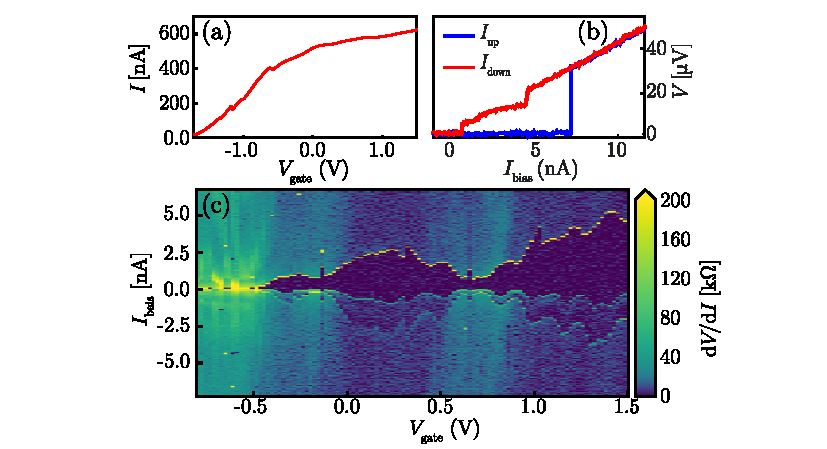
\includegraphics[width=\textwidth]{sup_fig1.pdf}
\caption{(a) Device current as a function of gate voltage, $V_\mathrm{bias}$ = 10 mV. Except the gate that is varied in this scan, other gates are at +3 V. (b) Voltage-current characteristic for both upwards (blue) and downwards (red) sweeping direction of current bias. The supercurrent of 8 nA is the maximum supercurrent observed in this device and corresponds to all gates at +3V. (c) Numerical derivative $\mathrm{d}V/\mathrm{d}I$ of $V\left(I\right)$ as function of current and gate voltage. Current bias is swept from negative to positive.}
\label{fig: charaterization_D1}
\end{figure}

Characterization of device 2 at $B$=0 T is shown in Figure \ref{fig: charaterization_D1}, devices 1 and 3 behave similarly (data not shown).
Current versus local gate voltage is measured at $V_{\text{bias}}$ = 10 mV (Figure \ref{fig: charaterization_D1}(a)). 
Taking known series resistances into account, the device resistance of $\sim$6 k$\Omega$ is found, corresponding to the sum of the conduction channels and contact resistances.

As shown in Figure \ref{fig: charaterization_D1}(b), by optimizing the gate voltages a maximal supercurrent of 8 nA was found, with a corresponding voltage of 32 $\mu$V, which developed upon switching to the normal state. 
The junction is hysteretic as shown by the low retrapping current, and has a sharp transition to the normal state, indicating that the junction is in the underdamped regime. 
Note that self-heating may also contribute to the hysteresis \cite{pekola2008hysteresis}. 


\section{Shapiro step measurements}

\begin{figure}[!h]
\centering
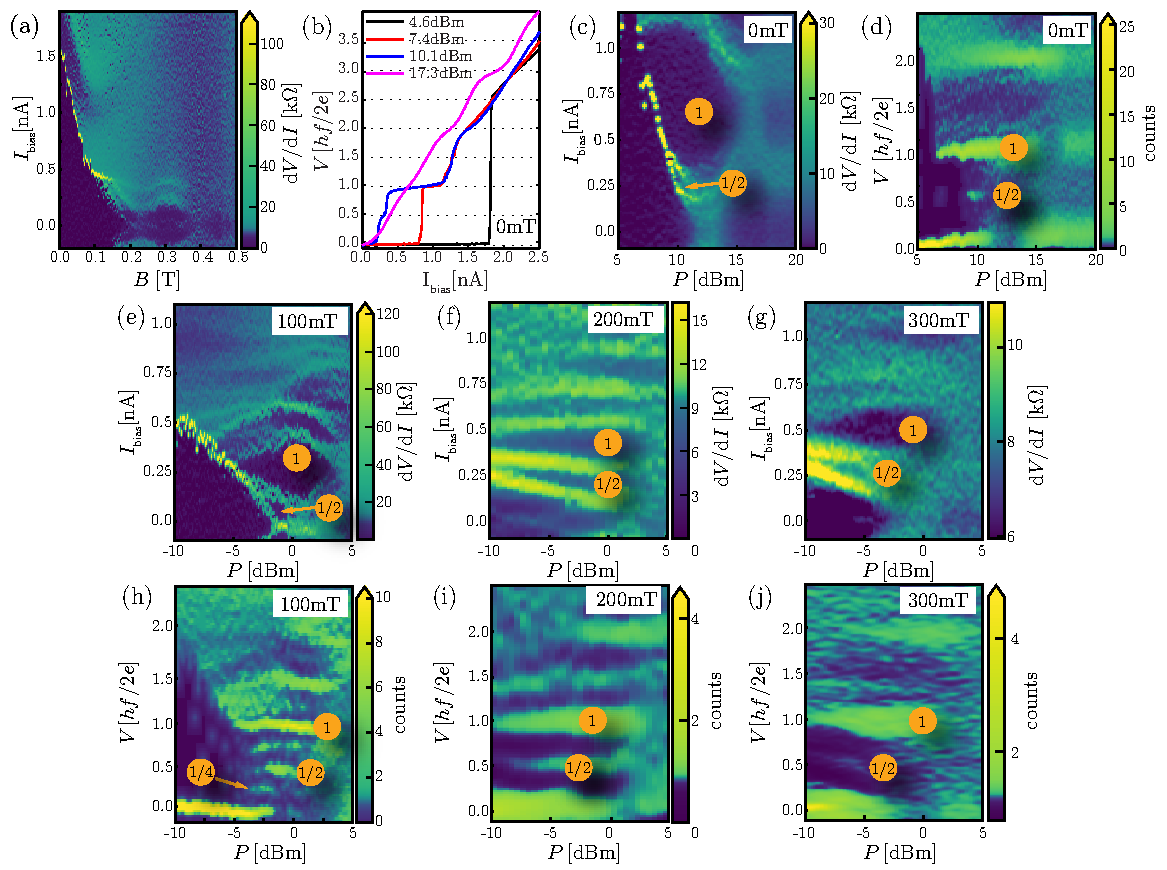
\includegraphics[width=\textwidth]{sup_fig2}
\caption{
Shapiro steps in magnetic field. 
(a) $B$ dependence of supercurrent without microwave radiation applied. 
Numerical derivative $\mathrm{d}V/\mathrm{d}{I}$ of the original $V\left(I\right)$ curves is shown. 
(b) Shapiro steps at $B = \SI{0}{\tesla}$ for different microwave powers. 
At the lowest RF power of 4.6 dBm (black line) no Shapiro steps are present. 
A half integer step is visible at 10.1 dBm (blue line). 
(c),(e)-(g) Microwave power dependence of Shapiro steps for different $B$. Numerical derivative $\mathrm{d}V/\mathrm{d}{I}$ of the original $V\left(I\right)$ curves is shown, in this representation the Shapiro step plateau corresponds to low differential resistance (blue color).
(d), (h)-(j) are Shapiro steps for different $B$ as a function of microwave power plotted in histogram. High voltage counts correspond to the plateaus in the Shapiro steps.
At $B = \SI{0}{\tesla}$ [panel (c)], the power dependence is dominated by integer Shapiro steps and only a small contribution of half integer steps is visible. 
At $B = \SI{100}{m\tesla}$ [panel (e)]  fractional steps are visible. Noticeably, not only half integer steps, but also quarter steps are weakly present in panel (h). 
$B = \SI{200}{m\tesla}$ [panel (f)] is closest to the minimum supercurrent at \SI{250}{m\tesla}. Here the half integer and integer steps are almost equal in width. 
Finally, beyond the minimum of supercurrent, at $B = \SI{300}{m\tesla}$ [panel (g)], the integer steps increase again in width relative to the half integer step.
Curves in (b) are from the same dataset as shown in (c). 
Values given for the RF power in panels (b)-(j) are the output power of microwave source, \SI{60}{\deci \bel} attenuation, of which \SI{20}{\deci \bel} at low T, is applied. 
Data is from device 2, second cooldown.}
\label{fig: shapiro}
\end{figure}

Device 2 has been cooled down a second time with a microwave antenna near the sample. 
This enabled the study of Shapiro steps in the junction as a function of microwave power and frequency, see Fig.~\ref{fig: shapiro}.
The device is again tuned to a multi-mode regime, comparable to $V_\mathrm{gate}$ = 0.5 V in Fig.~\ref{fig: charaterization_D1}(c). 
Due to an increased microwave background noise in the vicinity of the junction upon adding the antenna, an extra rounding of the $V\left(I\right)$-trace near the switching bias is present. 

Figure \ref{fig: shapiro}(a) is a magnetic field $B$ dependence of supercurrent in the absence of microwave drive. 
The supercurrent pattern as a function of $B$ is similar to the one shown in Figure 2 of the main text. 
This indicates that thermally cycling the device did not change the qualitative behavior of the device, although the exact gate tunings are different. 

We focus on the power dependence of Shapiro steps at different $B$ strengths of 0mT, 100mT, 200mT and 300 mT corresponding to Fig.~\ref{fig: shapiro}(c), (e), (f), (g) respectively. 
The microwave frequency is kept fixed at 2.0 GHz. Shapiro steps show up at voltages corresponding to $V=n\cdot\frac{hf}{2e}$, where $n$ may be a fraction. At $B$ = 0 mT [Fig.~\ref{fig: shapiro}(c)], half integer steps are only weakly present. 
At $B$ = 100 mT [Fig.~\ref{fig: shapiro}(e)], not only $n$ = 1/2 steps but also weak $n$ = 1/4 steps are visible (not marked with circled number). 
This is clearly visible in Fig.~\ref{fig: shapiro}(h), where the same data is plotted in a voltage histogram, with high voltage counts corresponding to the plateaus of the Shapiro steps.

The $B$ = 200 mT and $B$ = 300 mT cases [Fig.~\ref{fig: shapiro}(f), (g)] correspond to low critical currents. Nevertheless, Shapiro steps can still be resolved. At B = 200 mT, which is closest to the minimum of critical current, the width of the 1/2 step is more than half the width of the 1st step, and it is similarly large compared to the 1st step at 300 mT. Fig.~\ref{fig: shapiro}(i), (j) are the histogram representations of Fig.~\ref{fig: shapiro}(f), (g).

Shapiro steps at fractional frequencies, especially the half-integer steps, have been previously observed in Josephson junctions under various conditions\cite{Lehnert1999fractional,Dubos2001fractional, dinsmore2008fractional,PhysRevLett.92.257005,PhysRevLett.97.067006}. 
For instance, they can arise due to Josephson coupling of higher orders accompanied by a non-sinusoidal current-phase relationship\cite{PhysRevB.63.214512}. 
In quasi-ballistic few-mode Josephson junctions the current-phase relation is expected to be non-sinusoidal, consistent with half-integer Shapiro steps observed here even at zero magnetic field. 
The higher order 1/4-steps are more exotic and deserve a deeper study in the future, though they may also originate from a non-sinusoidal current-phase relationship. 
Non-sinusoidal current-phase relationships are obtained within our model, see Fig. \ref{fig:CPR}. However, Fourier analysis of the simulation suggests that Shapiro steps at 1/3 the Josephson voltage should dominate over 1/4 steps. This discrepancy remains not understood.

In a non-sinusoidal Josephson junction tuned to the $0-\pi$ transition the first order Josephson effect which is responsible for strong integer Shapiro steps vanishes, thus the current phase relationship is dominated by higher harmonics. 
In this case, Shapiro steps at half-integer and integer frequencies are expected to appear with the same step widths. 
The results presented here show that the ratio of step widths for half integer to integer steps indeed increases near a field-induced node in the critical current. However, the results are not conclusive as to whether this is due to a $0-\pi$ transition.

On the other hand, Majorana zero modes coupled across a junction barrier are predicted to result in disappearing odd-integer Shapiro steps\cite{lutchyn2010majorana,oreg2010helical}. 
Thus the behavior observed here is opposite to that expected due to Majorana modes: extra fractional steps in addition to integer steps are observed.

\newpage
\section{Angle dependence of fluctuations}
\onecolumngrid
In this section we present results from device 3 [Fig.~\ref{fig: SEM_D1D3}(c)] with contact spacing of 150 nm on which we performed current bias measurements with similar conditions as reported in the main text. 
Device 3 is fabricated with similar methods as Device 1 and 2, with the exception that $\text{HfO}_x$ is used as the dielectric material instead of $\text{SiN}_x$.

\begin{figure}[h]
\centering
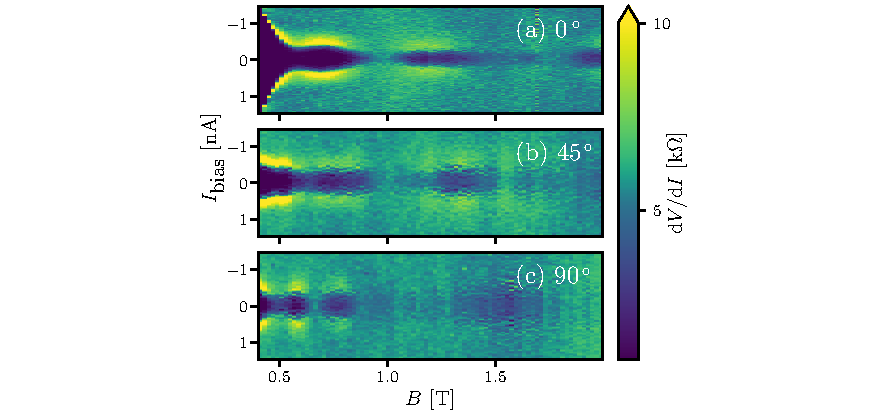
\includegraphics[width=\textwidth]{sup_fig3}
\caption{Differential resistance measured as a function of current bias and magnetic field strength of Device 3. The angle indicated in each panel is the angle of the magnetic field relative to the wire axis, in the plane of the substrate.}
\label{fig:angle_dependence}
\end{figure}

The device shows a monotonic decrease of the critical current for magnetic field values up to 400 mT (not shown in the figure). This extended initial decay is attributed to the shorter contact separation, and hence reduced influence of disorder on intermode interference. 

Beyond 400 mT, the critical current fluctuates at a period depending on the direction of the magnetic field. 
Figure \ref{fig:angle_dependence} shows the differential resistance of the device for three different field directions. 
The top panel shows data where the field is pointed along the nanowire. 
The critical current decays until the field reaches 600 mT, beyond which it exhibits a weakly pronounced maximum and disappears at 900 mT after which it reappears again. 
As the field angle is rotated in the plane of the substrate [Figs.~\ref{fig:angle_dependence}(b),(c)], the critical current decays faster as a function of the field strength, and the subsequent nodes of the critical current are closer spaced in field. 
We associate this behavior with increased flux through the nanowire at finite angles between the field and the wire.

\begin{figure}[!h]
\centering
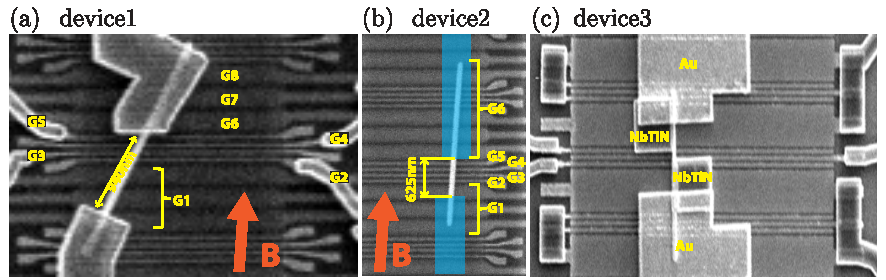
\includegraphics[width=\textwidth]{sup_fig4.pdf}
\caption{Schematics based on SEM picture of device 1, device 2 and device 3. 
(a) Device 1, with an angle of $25^{\circ} \pm 5^{\circ}$ with the magnetic field. 
In all devices, not all local gates are operated independently: as indicated in the figures, larger gates are formed by shorting some of the local gates together, e.g G1. 
(b) Device 2, shown with the superconducting electrode design superimposed on top of the SEM image, as this device has not been imaged after the final fabrication step. 
The device has a contact spacing of $\sim \SI{625}{nm}$, with the wire at an angle of $0^\circ \pm 5^\circ$ with respect to magnetic field. 
(c) Device 3, incorporating two quasi-particles traps (Au) next to the superconducting contacts. 
The length of the Josephson junction is $\sim \SI{150}{\nano \meter}$. 
Device 3 is cooled down in a setup where the magnetic field could be rotated using a 3D vector magnet.}
\label{fig: SEM_D1D3}
\end{figure}

\newpage

\section{Zero bias peaks due to supercurrent can onset at finite magnetic field}

If the Josephson junctions are tuned into the topological regime, devices used in this study can also support Majorana fermions. 
As a matter of fact, such a design is employed by several groups for the purpose of searching for Majorana zero modes. 
Here we show that such Josephson junction based devices, even if the contacts are almost \SI{1}{\micro \meter} apart, cannot be used for unambiguous detection of Majorana zero modes \cite{deng2012ZBP, deng2014parity, Harlingen2013ZBP}. 
Specifically, we observe that, in a voltage-biased measurement, supercurrent can appear as a zero-bias peak that onsets at a finite magnetic field, in the same range of parameters as those used in Majorana experiments, thus mimicking a key Majorana signature.

Figure \ref{fig: supercurrentZBP} shows the results. 
By applying a negative voltage to one of the local gates in between the superconducting contacts, a tunneling regime comparable to $V_\mathrm{gate}$ < -0.5 V shown in Figure \ref{fig: charaterization_D1}(a) for device 2 is achieved. 
The result of a current biased measurement in this regime is shown in Figure 5(a), a very small (down to 1 pA) supercurrent could be resolved. 
Interestingly, for gate regimes with lower resistance the supercurrent initially grows as expected, but then the $\mathrm{d}V/\mathrm{d}I$ peak related to the switching current broadens and is no longer visible. 
Here, we focus on the $B$ dependent behavior as shown in Figure \ref{fig: supercurrentZBP}(b),(c),(d) at a gate voltage indicated by the yellow line in Figure \ref{fig: supercurrentZBP}a. 
At $B=\SI{0}{T}$, no supercurrent was resolved in a current biased measurement, but upon increase of magnetic field, at around 200 mT, a small supercurrent shows up in a slightly more resistive regime. 
Such a small supercurrent may show up in a differential conductance measurement as a small zero bias peak (ZBP). 
Indeed, upon switching to a voltage biased differential conductance measurement, a small ZBP with height $\sim 0.01\frac{2e^2}{h}$ is found. 
Note that the ranges in which the supercurrent is visible in a current biased measurement and in which the ZBP is visible in a voltage biased measurement are not identical due to a minor charge switch between the two measurements.

\begin{figure}[!h]
\centering
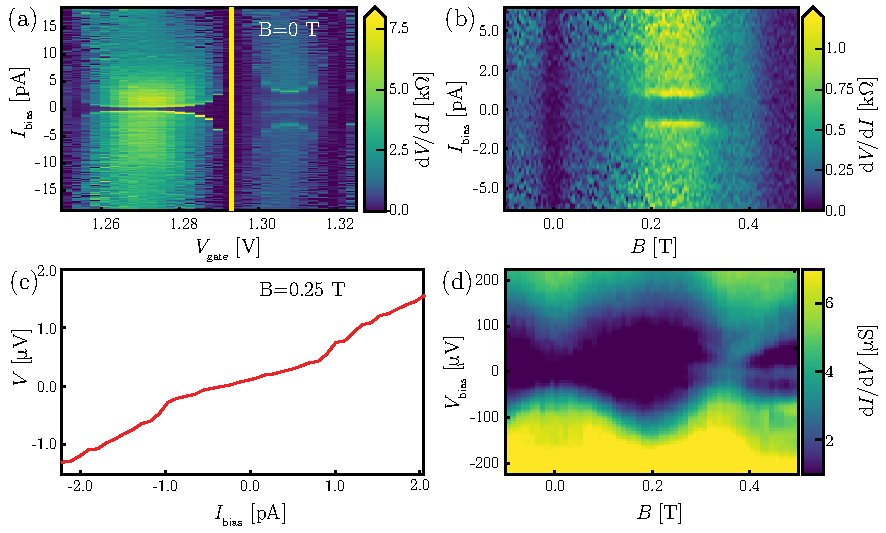
\includegraphics[width=\textwidth]{sup_fig5}
\caption{Supercurrents and zero bias peaks at finite $B$.
(a) Differential resistance vs gate. In this scan, one of the local gates is set at -0.45 V and all other gates are at +1.5 V.
(b) Differential resistance vs $B$ at the indicated gate position in (a).
(c) Linecut from (b) at $B = \SI{0.25}{T}$. (d) Differential conductance vs $B$ corresponding to (b). Numerical derivative of original $V\left(I\right)$ curves is shown in (a) and (b). Data from device 1.}
\label{fig: supercurrentZBP}
\end{figure}

\section{Extracting switching current from experimental data}

To obtain Fig. 5(a) of the main text, switching currents are extracted from a large set of voltage-current characteristics by numerically detecting the voltage step upon switching from the superconducting to the resistive regime. 
First, an initial low-pass filter is applied to the data reducing spurious fast fluctuations.
Next, a numerical derivative of the $V\left(I\right)$-curve is taken. 
This first derivative has a clear maximum for an $V\left(I\right)$-curve with a sharp transition, allowing for straightforward identification of the switching current.
However, the finite $B$-field $V\left(I\right)$-curves typically display smooth transitions from the superconducting to the resistive state, resulting in unclear or even absent maximums in the first derivative. 
A smooth transition still generates a maximum of the second derivative, allowing for identification of the switching current. 
We, therefore, introduced a threshold for a first derivative maximum, below which a second derivative is taken of the $V\left(I\right)$-curve with its maximum identified as the switching current.
A second threshold is introduced for the maximum of the second derivative, below which the switching current is considered to be zero. 
Algorithm parameters are optimized to both correctly identify the sharp transitions of large switching currents and to avoid false positives of small switching current. 


\section{Details of the modeling}

We discretize the Hamiltonian (1) of the main text on a cubic lattice with a lattice constant of $a=\SI{8}{nm}$.
The nanowire cross section has a diameter of $\SI{104}{nm}$ and the superconductor on top of the semiconductor nanowire adds two more layers of unit cells partially covering the nanowire ($135^{\circ}$ of the wire's circumference). There are 3 free parameters in the simulation for obtaining the correct induced gap in the nanowires, namely the coverage angle of the superconductor, the tunnel barrier between the SC and the SM, and the superconducting gap. The coverage angle is fixed at $135^{\circ}$ in order to save computational time. Since the Meissner effect is not included in the simulation, the exact value of the angle does not play a critical role. The superconducting order parameter $\Delta$ is set such that the induced gap inside the nanowire at zero field is $\Delta_\textrm{ind} = \SI{0.250}{meV}$.

The superconductor has the same lattice constant and effective mass as the nanowire, justified by the long-junction limit.
This means that the wave function has most of its weight in the nanowire and that the superconducting shell merely serves as an effective boundary condition that ensures that all particles are Andreev-reflected.
Further, the superconductor lacks the Zeeman effect and spin-orbit interaction. Zeeman effect in the superconductor is neglected because the g-factor in NbTiN is 2, much smaller than the g-factor in InSb (which is 50). 
We use realistic parameters of an InSb nanowire~\cite{mourik2012signatures}:  $\alpha=\SI{20}{\meV\cdot\nm}$, $m^{*}=0.015 m_e$, and $g=50$. 

The geometry of the modeled system is shown in Fig.~\ref{fig: system}.

\begin{figure}[!h]
\centering
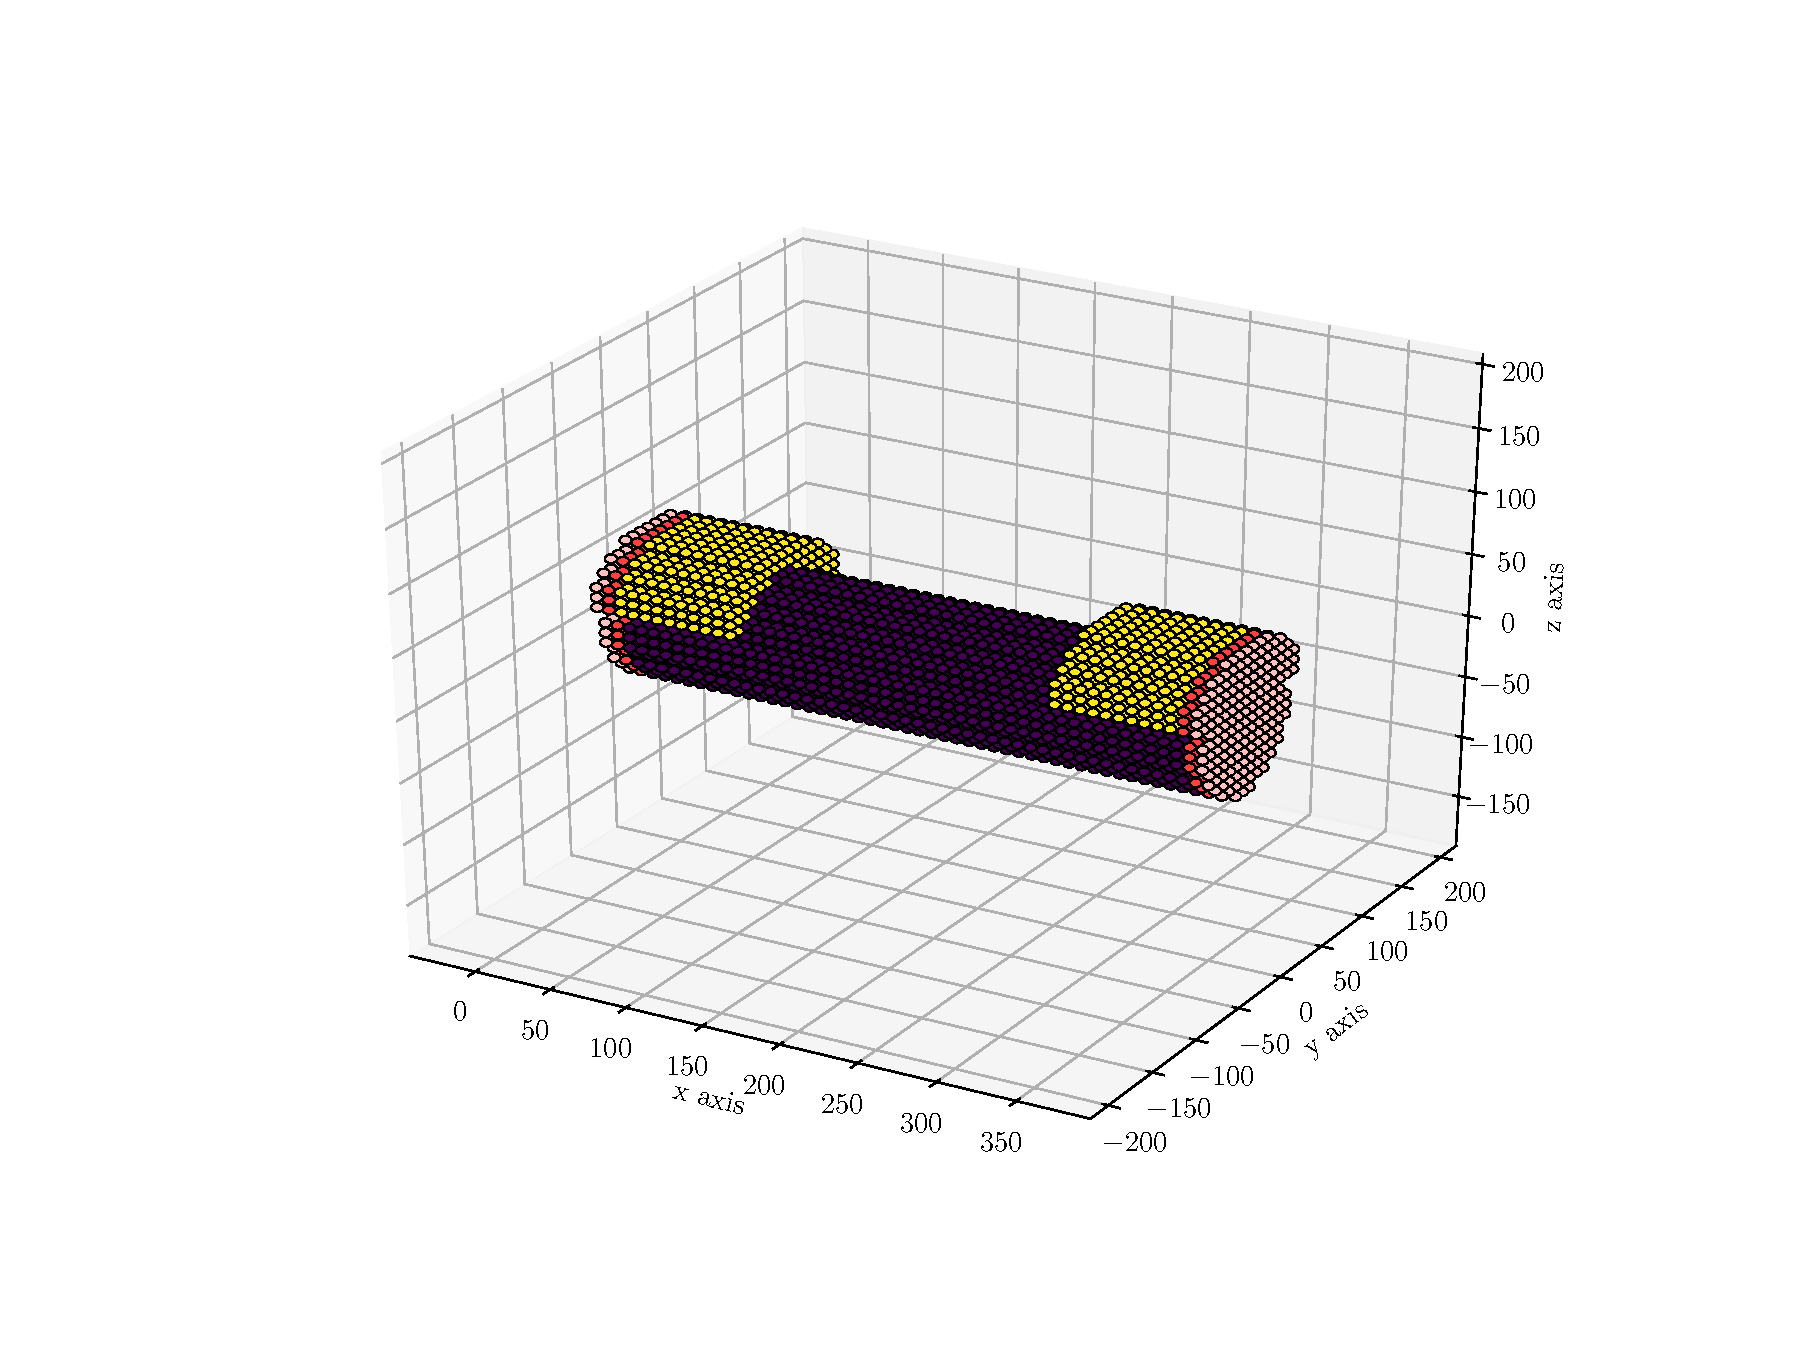
\includegraphics[width=\textwidth]{sup_fig6}
\caption{The modeled tight-binding system.
The purple sites indicate the semi-conductor and the yellow sites show the superconductor.
The red and light red colored cross sections indicate that the wire extends infinitely in that direction.
We defined the length of the wire $L$ as the part that is not covered with the superconductor. In this figure for clarity we plot a shorter wire ($L=\SI{200}{\nm}$), while in the simulations we chose $L=\SI{640}{\nm}$.
The other dimensions used in the simulations are as depicted. 
Specifically, the wire diameter is $\SI{104}{\nm}$, the thickness of the superconductor is $16-\SI{24}{\nm}$, and the coverage angle of the superconductor is 135$^{\circ}$.}
\label{fig: system}
\end{figure}

\section{Detailed theoretical estimates}
In this section we estimate the strength of different possible mechanisms that can cause supercurrent fluctuations in the nanowire Josephson junction.

\textit{Interference between orbital channels}.
The area of the cross section of the nanowire is $\sim \pi \times (\SI{50}{nm})^2$. This means that the magnetic field value of $B \approx \SI{0.26}{T}$ corresponds to one flux quantum penetrating the cross section of the nanowire.
At this value of the magnetic field we expect the phase shifts between different bands propagating between the two superconductors to be comparable to $\pi$.
This sets the typical $B$ scale for the interference of different orbital modes carrying current, which is well within the experimentally observed typical difference in $B$ of consecutive critical current minimums.
This simple estimate neglects the magnetic field expulsion of the superconductor, which may create a higher flux in the nanowire near the superconducting contacts, thus lowering the effective field scale.

These estimates are similar to the analysis for the Fraunhofer-like interference in diffusive many-channel junctions\cite{Cuevas2007}. The novelty is, however, in the small number of channels in our junction, which causes irregular interference instead of the regular Fraunhofer pattern in the former case. Another important observation in our case is that even though the magnetic field is along the junction, it can still cause the interference due to different transverse profiles of the propagating modes.\\

\textit{Interference between spin channels}.
Supercurrent fluctuations can be produced by $0-\pi$ transitions due to the Zeeman splitting of the Andreev bound states inside the Josephson junction.
The characteristic $B$ scale of such supercurrent fluctuations is determined by the ratio of Zeeman energy to the Thouless energy.
This sets the relative phase $\theta_\mathrm{B}$ of the Andreev bound states, $\theta_\mathrm{B} = E_\mathrm{Z} L / \hbar v_\mathrm{F}$.
Here $E_\mathrm{Z}$ is the Zeeman energy, $L$ the length of the nanowire junction, and $v_\mathrm{F}$ the Fermi velocity in the nanowire.
The junction undergoes a $0-\pi$ transition when the relative phase difference of the ABS $\theta_\mathrm{B}$ reaches the value $\pi/2$. Such a transition is marked by a minimum in the junction critical current as a function of $B$.
Since $v_\mathrm{F}\approx \sqrt{2\mu / m^*}$, the field value at which $\theta_\mathrm{B}=\pi/2$ depends on the chemical potential $\mu$.
We thus estimate the upper bound of the magnetic field at which the first $0-\pi$ transition occurs by assuming a maximal value of $\mu \sim \SI{15}{meV}$ corresponding to the intermode spacing\cite{vanweperen2015spinorbit,kammhuber2016conductance}.
Assuming a junction length of $L=\SI{1}{\micro\meter}$, the upper bound of the transition occurs at $B\sim \SI{0.5}{T}$.
Generally, for smaller $\mu$, this value is significantly lower, therefore purely Zeeman induced supercurrent fluctuations are well within the range of our experiment.
These estimates are confirmed in our numerical simulations, see $\alpha=0$ lines of Fig.~\ref{fig:currents_1D_alpha_vs_B_x}.

\textit{Interference between spin, Zeeman and spin-orbit}.

\begin{figure}
\centering
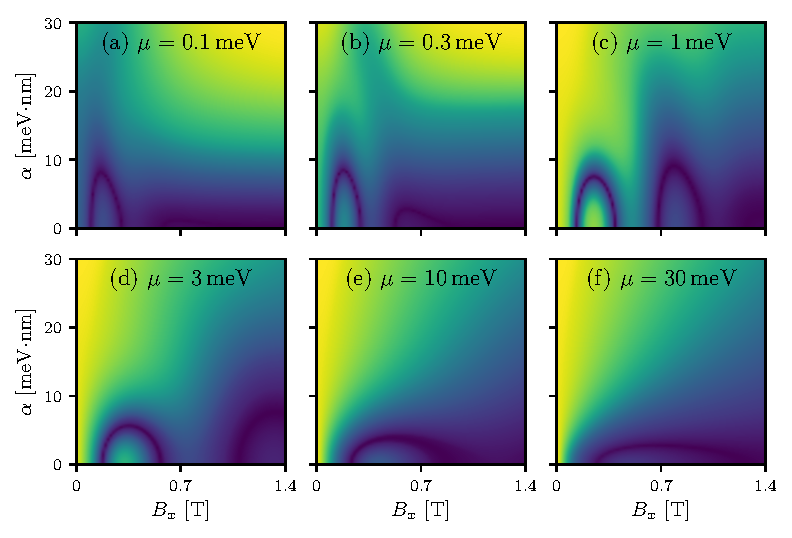
\includegraphics[width=0.75\textwidth]{sup_fig7}
\caption{Critical currents in a simple one-channel toy nanowire model\cite{lutchyn2010majorana,oreg2010helical} as a function of spin-orbit coupling strength $\alpha$ and magnetic field along the wire $B_x$.
The different panels (a)-(f) are taken at different chemical potentials, $0.1,\; 0.3,\; 1,\; 3,\; 10,\; \SI{30}{meV}$ respectively.
The color scales are not normalized across the different panels, but are all separately scaled to optimally show all features in every plot.
We observe how the $0-\pi$ transitions at finite $B_x$ get mutually annihilated upon increasing $\alpha$.\label{fig:currents_1D_alpha_vs_B_x}}
\end{figure}

The previous discussion on spin related interference considered the Zeeman effect only.
However, the strong spin-orbit interaction in the nanowire fixes the spin direction to the propagation direction and thus counteracts the effect of the Zeeman splitting. 
Following Ref.~\onlinecite{yokoyama2014anomalous}, the characteristic parameter for spin-orbit is $\theta_{SO} = \frac{\alpha k_\mathrm{F} L}{\hbar v_\mathrm{F}} = \frac{\alpha m^* L}{\hbar^2} = L/L_\mathrm{SO}$.
Here $L_\mathrm{SO}$ is the spin-orbit length, which is expected to be in the $50-\SI{250}{nm}$ range, much shorter than $L$.
For the Zeeman effect to cause a $0-\pi$ transition it needs to overcome the spin-orbit spin quantization. 
This means that the spin-orbit term increases the field at which the first $0-\pi$ transition happens, and this increase is stronger as the chemical potential is further away from the band bottom.
This interplay between Zeeman and spin-orbit interaction is expected to be highly anisotropic\cite{yokoyama2014anomalous} in the direction of $B$; the scenario described above assumes the external $B$ field and effective spin-orbit field to be perpendicular, as is expected for applying $B$ along the nanowire axis.
To substantiate our estimates we have used a nanowire toy model\cite{lutchyn2010majorana,oreg2010helical} to obtain critical current as a function of gate voltage, magnetic field, and spin-orbit coupling in Fig.~\ref{fig:currents_1D_alpha_vs_B_x}.
The model indeed illustrates that the further the chemical potential is from the bottom of the band the higher is the value of the magnetic field at which the $0-\pi$ transition occurs. 

In summary, the above estimates suggest that orbital interference is present regardless of the exact value of $\mu$, whereas spin related interference is highly restricted in $\mu$ range.
This favors an orbital interference interpretation of the experimental observations, since the supercurrent variations in the experiment are always present in a similar field range no matter the exact gate potential.

To illustrate this reasoning we produced Fig.~\ref{fig:currents_1D_alpha_vs_B_x}, which shows supercurrent fluctuations as a function of the distance to the bottom of the band in a single-band wire. With increasing the distance to the bottom of the bands $0-\pi$ transitions happen at higher fields. Upon ramping up spin-orbit strength the $0-\pi$ transitions disappear.

\section{Current phase relations and Josephson energies}
\begin{figure}[!h]
\centering
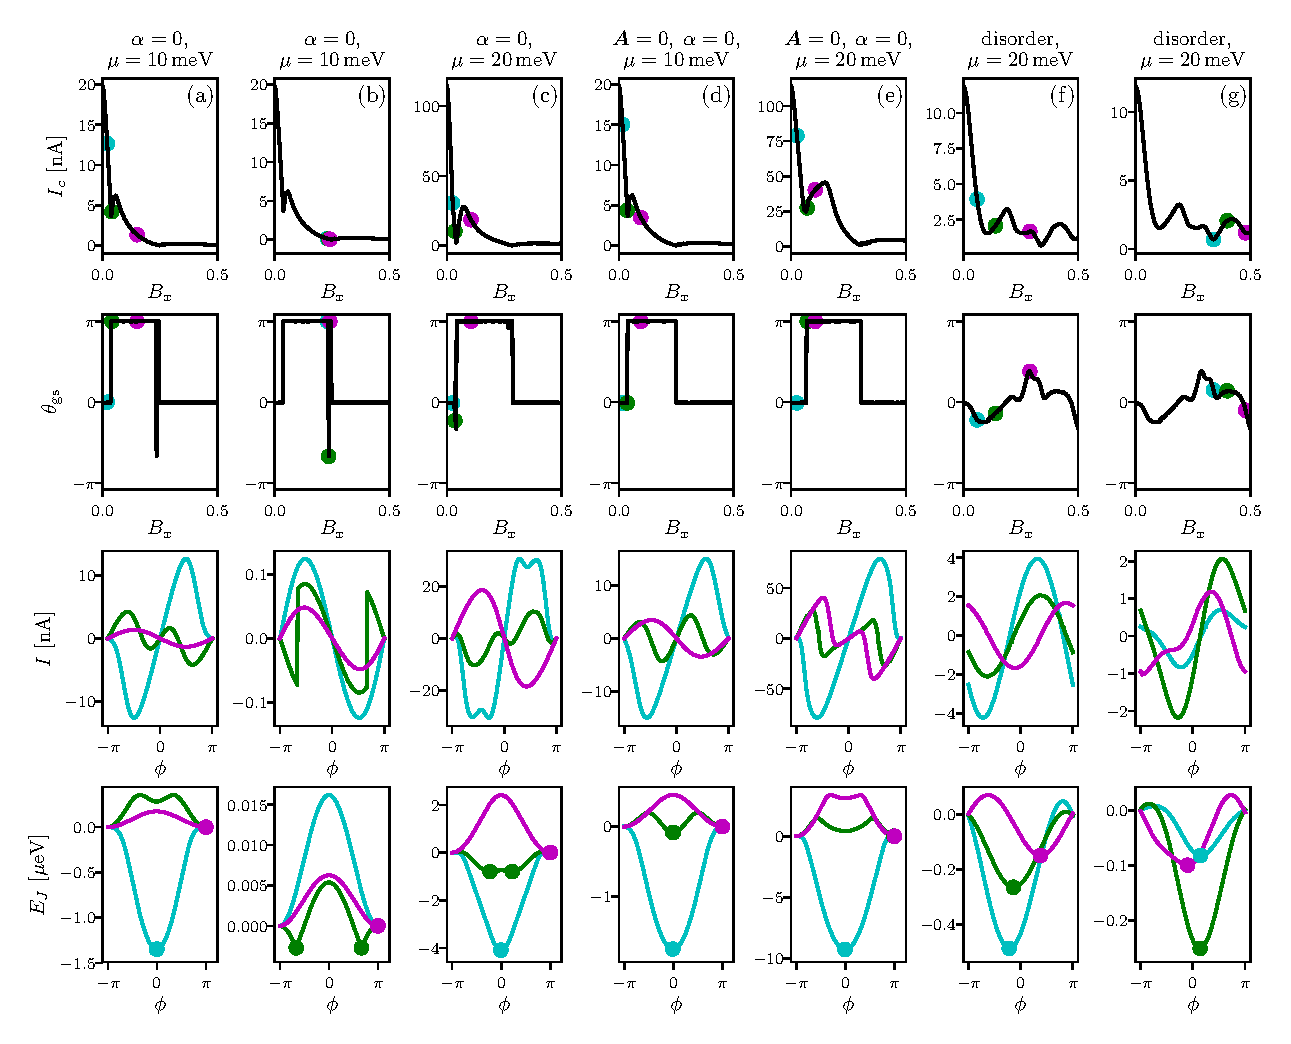
\includegraphics[width=\textwidth]{sup_fig8.pdf}
\caption{(a)-(g) The critical current and ground state phase difference as function of magnetic field, and current phase relations (CPRs) and Josephson energies as functions of phase difference between the superconductors, for different parameters used in the model as labeled.
From top to bottom: $I_c(B_x)$ and $\theta_{\textrm{gs}}$ with the three points indicating the magnetic field values for which the CPR and $E_J(\phi)$ are plotted; CPRs for the three values of magnetic fields; Josephson energies as functions of the phase difference.
The dot in the bottom row $E_J$ indicates the energy minimum and the ground state phase difference.
Note that identical model parameters are used in columns (a),(b) and (f),(g) respectively, but different consecutive junctions states of interest are highlighted in the individual columns. 
\label{fig:CPR}}
\end{figure}

To further support the claims of the previous section and to discuss the role of the ground state phase, we plot the evolution of the critical current and the ground state phase difference with magnetic field, and show the current-phase relations and Josephson energies characteristic for each junction state in Fig.~\ref{fig:CPR}.
$0-\pi$ transitions happen in the absence of spin-orbit interaction (Fig.~\ref{fig:CPR}(a)-(e)). 
In the presence of spin-orbit and disorder, due to breaking of the spatial symmetry the ground state phase can obtain any single value $\varphi_0$ (a so-called $\varphi_0$-junction) near the crossover between $0$ and $\pi$ states of the junction ((Fig.~\ref{fig:CPR}(f)-(g)).
Note that without disorder, the spatial mirror symmetry with respect to the middle of the system forces all CPRs $I(\phi)$ to be odd functions and all $E_J(\phi)$ to be even functions of $\phi$.
When spatial mirror symmetry holds, the junction's Josephson energy can still have a double minimum at $\pm\varphi$ (a so called $\varphi$-junction), thus $E_J(\phi)$ taking a Mexican hat type shape (green curves in (Fig.~\ref{fig:CPR}(b)-(c)).
However, because of this restriction imposed by spatial mirror symmetry, $\varphi$-junctions are rare and most junctions are either 0 or $\pi$-junctions.
Contrarily, including disorder breaks this symmetry leading to commonly occurring $\varphi_0$-junctions.

\section{Effect of disorder}

\begin{figure}[!h]
\centering
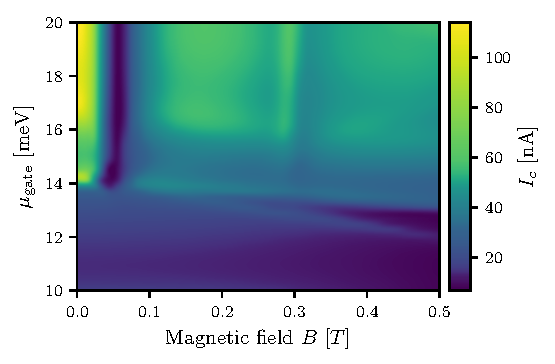
\includegraphics[width=0.75\textwidth]{sup_fig9.pdf}
\caption{Critical current as a function of the magnetic field and the gate voltage. The simulation parameters are identical to the ones used in Fig.~5 in the main text, but we set disorder to zero.\label{fig:gate_dependence}}
\end{figure}

Here we prove the essential effect of disorder on the supercurrent dependence on gate voltage.
We see the effect of disorder on $I_c(V_\textrm{gate})$ by comparing Fig.~5(b) of the main text and Fig.~\ref{fig:gate_dependence}, where we have switched off disorder.
In the clean case, where the main effect of the gate voltage on the supercurrent is via the gradual suppression of transmission through the nanowire, we observe that varying the gate voltage barely causes fluctuations of the supercurrent, even at finite magnetic field.
In the disordered case, changing the gate voltage effectively changes the realization of disorder in the region of the wire above the gate, thus causing supercurrent fluctuations. With the increased disorder, the dwell time in the gated region of the nanowire is increased, so the gate voltage dependence increases with reduced mean free path.
We found that no disorder and disorder with mean free path greater than the system size cannot explain the observed dependence of the critical current on magnetic field and gate voltage.

\section{Rotating magnetic field}
\begin{figure}
\centering
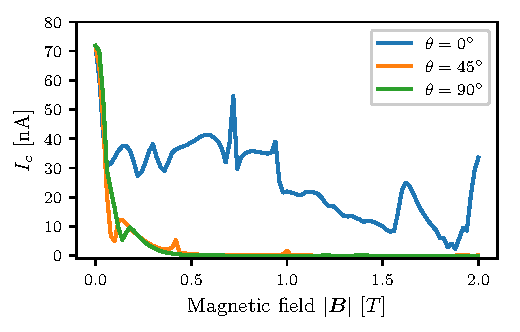
\includegraphics[width=0.75\textwidth]{sup_fig10}
\caption{
Supercurrent as a function of magnetic field for different directions of the applied field.
The angle is measured with respect to the wire axis and is rotated in the plane $\hat{x}$ parallel to the wire and $\hat{y}$ perpendicular to the wire and parallel to the substrate.
We use the same parameters as in Fig.~5 of the main text\label{fig:rotation_of_field}.
Besides the field purely along $\hat{y}$ the fluctuations pattern is qualitatively similar in all the directions.}
\end{figure}

Here we model the supercurrent fluctuations for different directions of the magnetic field, from parallel to the wire to perpendicular to it. 
The results of the modeling are in Fig.~\ref{fig:rotation_of_field}.
We see that for all directions of the field, besides one parallel to the wire, the fluctuation pattern is basically the same.
This is in accordance with the experimental observations of Fig.~\ref{fig:angle_dependence}. 

\bibliography{bibliography.bib}

\end{document}